\documentclass[parskip=full]{scrartcl}
\usepackage[top=2.54cm, bottom=2.54cm, left=2.54cm, right=2.54cm]{geometry}
\usepackage[utf8]{inputenc} % use utf8 file encoding for TeX sources
\usepackage[T1]{fontenc}    % avoid garbled Unicode text in pdf
\usepackage[ngerman]{babel}  % german hyphenation, quotes, etc
\usepackage{hyperref}       % hyperlinks in document
\usepackage{glossaries}     % glossary 
\usepackage{enumerate}      % advanced enumeration
\usepackage[shortlabels]{enumitem}
\usepackage[dvipsnames]{xcolor}
\usepackage{graphicx}
\usepackage{caption}        % add captions
\usepackage{adjustbox}      % add adjustmentbox
\usepackage{csquotes}

% Set footer and header bar
\usepackage[headsepline, footsepline]{scrlayer-scrpage}
\addtokomafont{headsepline}{\color{BlueViolet}}
\addtokomafont{footsepline}{\color{BlueViolet}}
\KOMAoptions{headsepline=1.25pt:\textwidth}
\KOMAoptions{footsepline=1.25pt:\textwidth}
\clearpairofpagestyles
\rofoot{\thepage}
\ihead{Write your own Android App: SpiceSquad}

% set the hyperlink style in the document
\hypersetup{
    pdftitle={PSE: Entwurfsheft},
    pdfborderstyle={/S/U/W 1},
    colorlinks,
    linkcolor={black!50!black},
    citecolor={blue!50!black},
    urlcolor={blue!80!black}
}

% sets right quotation for "
\MakeOuterQuote{"}

%change figure numbering
\renewcommand{\thefigure}{\thesection.\arabic{figure}}

%add command to hide subsections from toc
\newcommand{\changelocaltocdepth}[1]{%
  \addtocontents{toc}{\protect\setcounter{tocdepth}{#1}}%
  \setcounter{tocdepth}{#1}%
}

\newcommand{\enablesubsectionnumbering}[1]{
    \renewcommand{\thesubsection}{$\langle$#1\arabic{subsection}0$\rangle$}
    \changelocaltocdepth{1} 
}

\newcommand{\resetsubsectionnumbering}{
    \renewcommand{\thesubsection}{\arabic{section}.\arabic{subsection}}
    \changelocaltocdepth{3} 
}

% glossary
\makeglossaries
\renewcommand{\glossarysection}[2][]{}

\begin{document}
\newglossaryentry{label}{
    name=Label,
    plural=Labels,
    description={Rezepte können mit bezeichnenden Stichwörtern, sogenannten Labels, versehen werden. Dies ermöglicht das Filtern von Rezepten nach bestimmten Eigenschaften (z.B. vegetarisch, glutenfrei, halal)}
}

\begin{titlepage}
    \begin{center}
        \begin{Huge}
            {\textbf{Write your own Android App: SpiceSquad}}
        \end{Huge}
        \vspace{12px}

        Praxis der Softwareentwicklung (PSE)\\
        Sommersemester 2023\\
        \vspace{150px}

        \begin{Huge}
            {\textbf{Entwurfsheft}}
        \end{Huge}
        \vspace{12px}

        \textbf{Auftraggeber}\\
        Karlsruher Institut für Technologie\\
        KASTEL — Institut für Informationssicherheit und Verlässlichkeit\\
        \vspace{330px}

        \textbf{Auftragnehmer}\\
        Karlsruher Intellektuelle\\
        Henri Becker, Konrad Knappe, Lukas Schwarz, Raphael Zipperer\\
    \end{center}
\end{titlepage}

\tableofcontents
\newpage

\section*{Gender-Hinweis}
Zur besseren Lesbarkeit wird in diesem Entwurfsheft das generische Maskulinum verwendet.
Die in diesem Heft verwendeten Personenbezeichnungen beziehen sich – sofern nicht anders kenntlich gemacht – auf alle Geschlechter.
\newpage

\section{Einleitung}
Das Entfurfsheft des Projekts: "Write your own Android App: SpiceSquad" baut auf des zuvor verfasste Pflichtenheft auf.
Hierzu wurde zunächst ein umfassendes Klassendiagramm erstellt. Auf diesem basierend werden alle Klassen, Methoden und Attribute ausführlich erklärt.
In weiteren Kapiteln wird der REST-Webservice und die Datenbankstruktur beschrieben. Zum besseren Verständnis sind Ablaufbeschreibungen in Form von Sequenzdiagrammen angefügt.

\section{Struktur}

\subsection{Client-Server-Architektur}
Wie bereits im Pflichtenheft angeführt, haben wir uns für eine Trennung von Client und Server entschieden, um somit eine höchstmögliche Modularität zu gewährleisten und
Funktionen wie Squads zu ermöglichen. Die Kommunikation erfolgt über REST-Schnittstellen, welche eine einheitliche Schnittstelle mit dem Server bieten und eine einfache Skalierbarkeit begünstigen.
Im Folgenden werden die Architekturen von Server und Client näher beschrieben.

\subsection{Architektur der Applikation}
Für die Entwicklung der Applikation soll Flutter benutzt werden. Dies bietet einige Vorteile. Flutter ist ein plattformübergreifendes Framework, das es Entwicklern ermöglicht, eine einzige Codebasis zu verwenden, um Apps sowohl für iOS als auch für Android zu erstellen. Dies reduziert den Entwicklungsaufwand erheblich, da Entwickler nicht separate Codes für jede Plattform schreiben müssen. Flutter verwendet die Dart-Programmiersprache, die eine einfache Syntax und eine umfangreiche Bibliothek bietet, um leistungsstarke und ansprechende Benutzeroberflächen zu erstellen. Darüber hinaus verfügt Flutter über eine Hot-Reload-Funktion, die es Entwicklern ermöglicht, Änderungen in Echtzeit zu sehen, was den Entwicklungsprozess beschleunigt. Flutter-Apps sind schnell, reaktionsfähig und bieten eine extrem gute Leistung, da sie direkt auf die nativen Funktionen des Betriebssystems zugreifen. Diese Kombination aus plattformübergreifender Entwicklung, einfacher Sprache, schnellem Entwicklungsprozess und guter Leistung macht Flutter zur Wahl für die Entwicklung von SpiceSquad.

Die Applikation wird in vier große Schichten gegliedert. Dies dient dazu, die Bestandteile der App nach ihrer Funktion zu gruppieren und die Abhängigkeiten zwischen den einzelnen Komponenten zu minimieren. Dadurch wird die Wartbarkeit massiv verbessert und auch die Erweiterbarkeit der Applikation wird durch diese Strukturierung erleichtert. Die Schichten orientieren sich stark an den Empfehlungen von Google für die Architektur von Android Applikationen. Die vier Schichten sind der \textbf{Presentation Layer}, der \textbf{Application Layer}, der \textbf{Domain Layer} und der \textbf{Data Layer}.
\begin{figure}[htp]
    \centering
    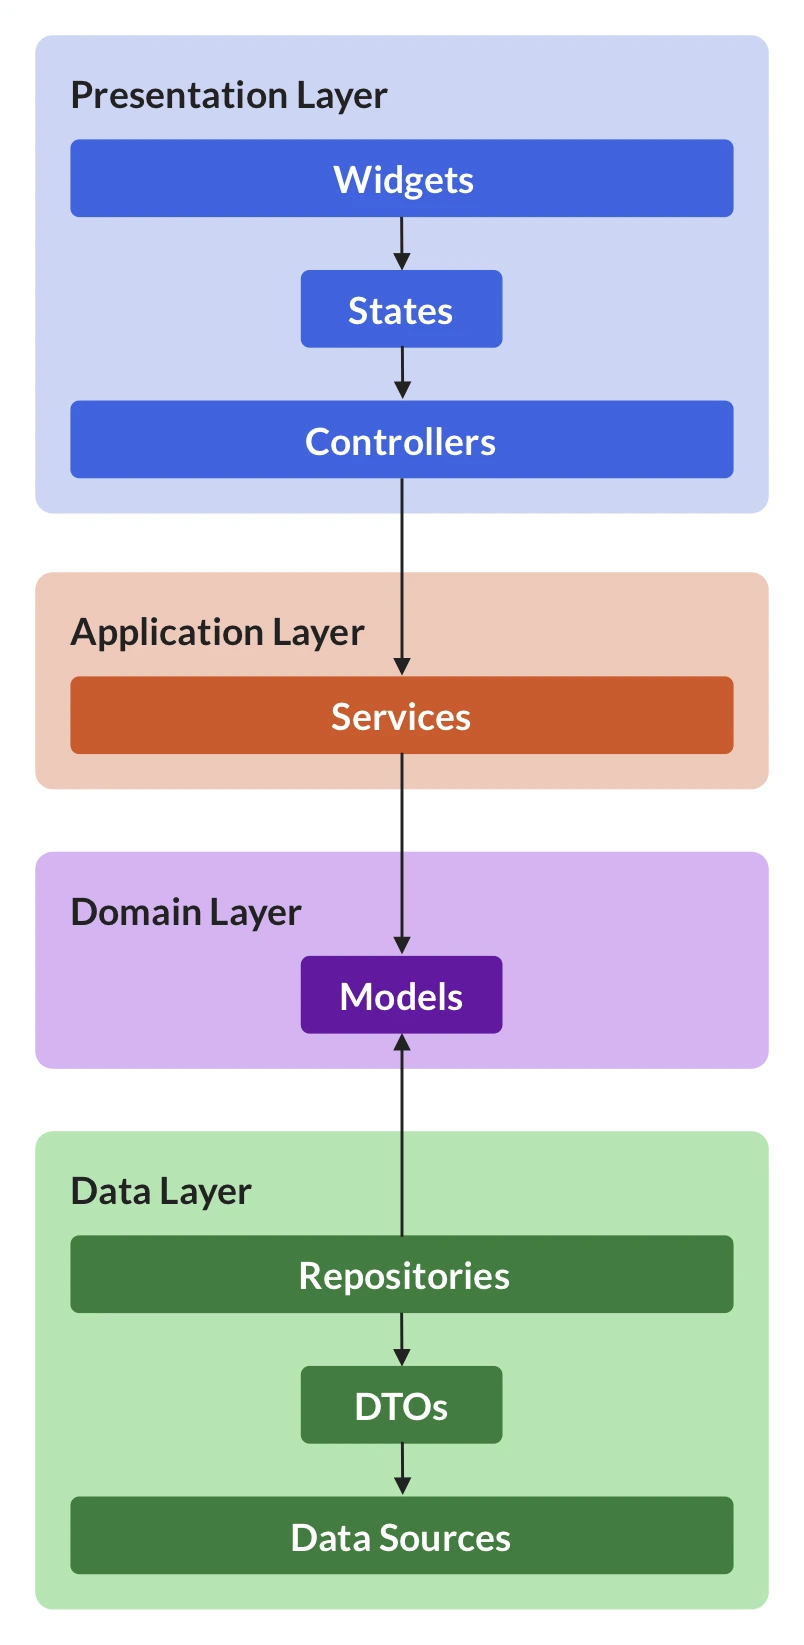
\includegraphics[height = 0.4\textheight]{images/architecture/architecture.png}
    \caption{Architektur der Applikation}
    \label{fig:struktur}
    %\footnotetext{Quelle: \url{https://codewithandrea.com/articles/flutter-app-architecture-application-layer/}}
\end{figure}
Die einzelnen Schichten werden in den folgenden Kapiteln genauer beschrieben.

\newpage

\section{Domain Layer}
\changelocaltocdepth{2}
\begin{figure}[htp]
    \centering
    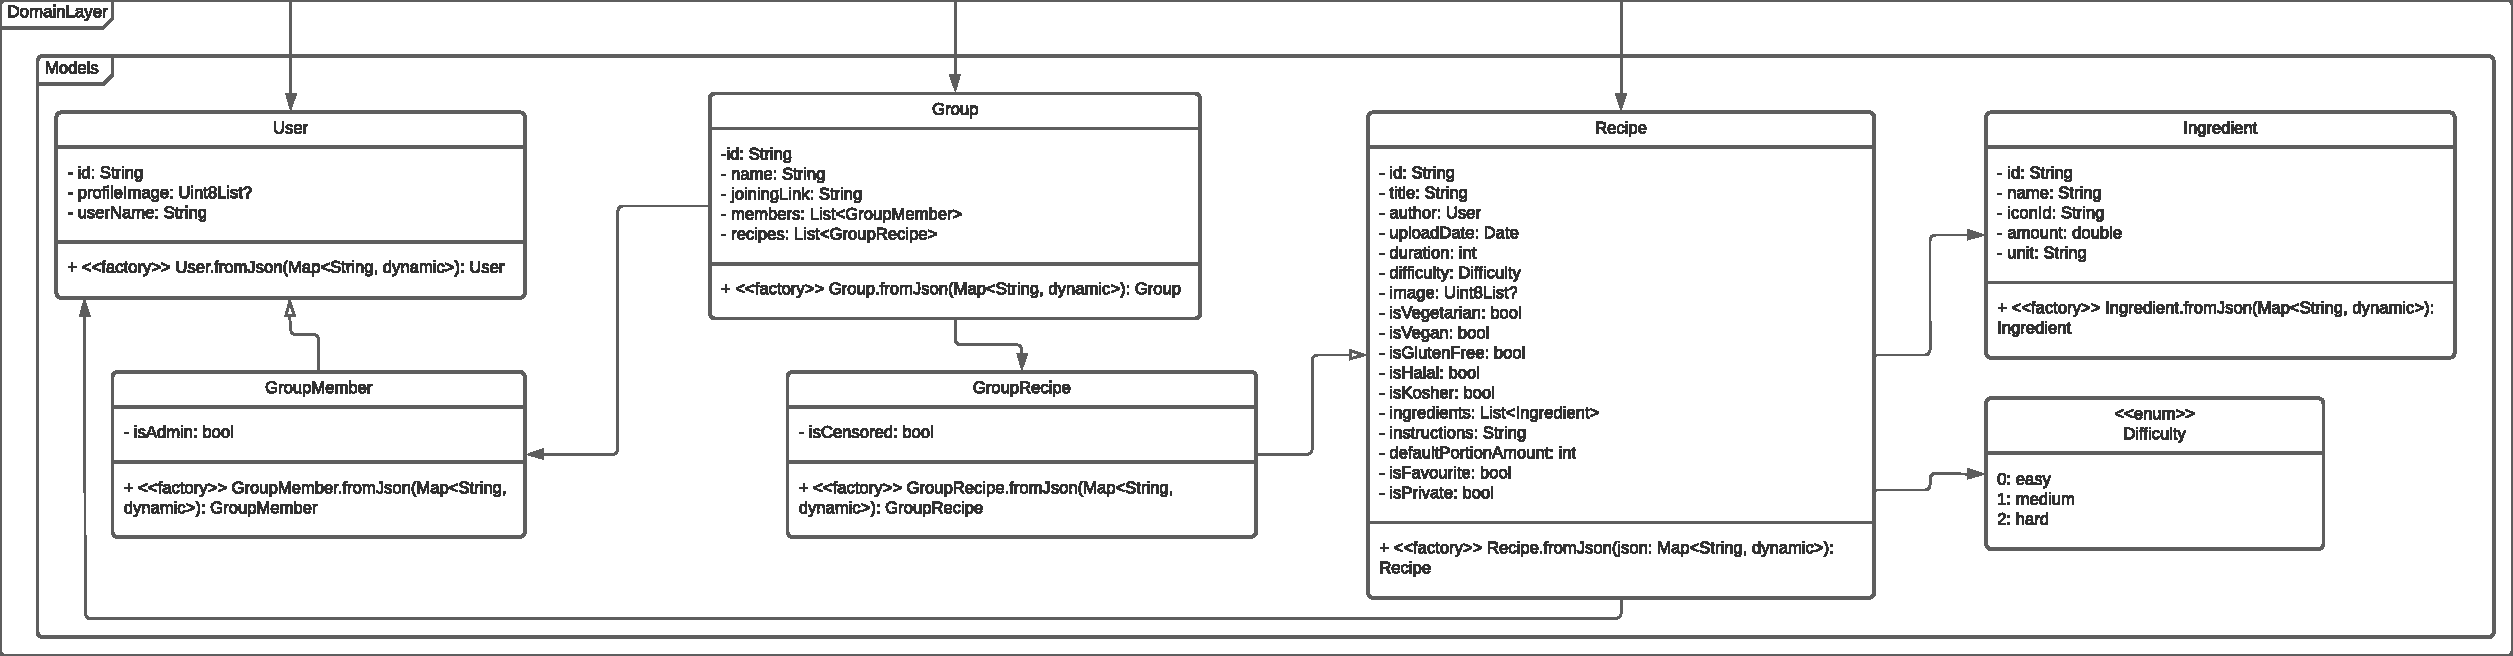
\includegraphics[width = \textwidth]{images/domainLayer/domainLayer.pdf}
    \caption{Klassendiagramm des Domain Layer}
    \label{fig:domain-layer}
\end{figure}
Der Domain Layer enthält in erster Linie die Models der einzelnen Entitäten. Diese sollen nun genauer beschrieben werden.
\subsection{User}
Die User-Klasse repräsentiert einen Nutzer der App.
\subsubsection{Attribute}
Alle Attribute sind privat und können nur über einen Getter gelesen werden.
\paragraph{profileImage: Uint8List?}
Das Profilbild des Nutzers. Der Typ Uint8List ist ein Array von Bytes, welches das Bild in binärer Form enthält. Dieses Attribut ist optional, da nicht jeder Nutzer ein Profilbild haben muss.
\paragraph{username: String}
Der Nutzername des Nutzers.

\subsubsection{Methoden}
\paragraph{getProfileImage(): Uint8List?}
Gibt das Profilbild des Nutzers zurück. Ist kein Profilbild gesetzt, wird null zurückgegeben.
\paragraph{getUsername(): String}
Gibt den Nutzernamen des Nutzers zurück.
\paragraph{factory User.fromJson(Map<String, dynamic> json): User} Factory-Methode zum Erstellen eines User-Objekts aus einem \glslink{JSON}{JSON-Objekt}. Sie wird verwendet, um die Daten, die vom Server geschickt werden und in \Gls{JSON} vorliegen, in ein User-Objekt umzuwandeln. Die Methode ist statisch, da sie kein User-Objekt benötigt, um aufgerufen zu werden. Nimmt als Parameter das bereits in eine Map umgewandelte \glslink{JSON}{JSON-Objekt} entgegen und gibt ein User-Objekt zurück.

\subsection{Recipe}
Die Recipe-Klasse repräsentiert ein Rezept.
\subsubsection{Attribute}
Alle Attribute sind private und können nur über Getter-Methoden abgerufen werden.
\paragraph{title: String}
Der Titel des Rezepts.
\paragraph{author: User}
Der Autor des Rezepts.
\paragraph{uploadDate: Date}
Das Datum, an dem das Rezept hochgeladen wurde.
\paragraph{duration: int}
Die Dauer zum Nachkochen des Rezepts in Minuten.
\paragraph{difficulty: Difficulty}
Die Schwierigkeit des Rezepts.
\paragraph{image: Uint8List?}
Das Bild des Rezepts. Der Typ Uint8List ist ein Array von Bytes, welches das Bild in binärer Form enthält. Dieses Attribut ist optional, da nicht jedes Rezept ein Bild haben muss.
\paragraph{isVegetartian: bool}
Gibt an, ob das Label "Vegetarisch" aktiviert ist.
\paragraph{isVegan: bool}
Gibt an, ob das Label "Vegan" aktiviert ist.
\paragraph{isGlutenFree: bool}
Gibt an, ob das Label "Glutenfrei" aktiviert ist.
\paragraph{isHalal: bool}
Gibt an, ob das Label "Halal" aktiviert ist.
\paragraph{isKosher: bool}
Gibt an, ob das Label "Koscher" aktiviert ist.
\paragraph{ingredients: List<Ingredient>}
Die Liste der Zutaten, die für das Rezept benötigt werden.
\paragraph{instructions: String}
Die Zubereitungsanleitung des Rezepts.
\paragraph{defaultPortionAmount: int}
Die Anzahl der Portionen, die das Rezept standardmäßig ergibt. Wird zum Berechnen der Mengen der Zutaten benötigt.
\paragraph{isFavourite: bool}
Gibt an, ob das Rezept vom Nutzer als Favorit markiert wurde.
\paragraph{isPrivate: bool}
Gibt an, ob das Rezept privat ist. Private Rezepte können nur vom Autor selbst gesehen werden.

\subsubsection{Methoden}
\paragraph{getTitle(): String}
Gibt den Titel des Rezepts zurück.
\paragraph{getAuthor(): User}
Gibt den Autor des Rezepts zurück.
\paragraph{getUploadDate(): Date}
Gibt das Datum, an dem das Rezept hochgeladen wurde, zurück.
\paragraph{getDuration(): int}
Gibt die Dauer zum Nachkochen des Rezepts in Minuten zurück.
\paragraph{getDifficulty(): Difficulty}
Gibt die Schwierigkeit des Rezepts zurück.
\paragraph{getImage(): Uint8List?}
Gibt das Bild des Rezepts zurück. Ist kein Bild gesetzt, wird null zurückgegeben.
\paragraph{getIsVegetarian(): bool}
Gibt zurück, ob das Label "Vegetarisch" aktiviert ist.
\paragraph{getIsVegan(): bool}
Gibt zurück, ob das Label "Vegan" aktiviert ist.
\paragraph{getIsGlutenFree(): bool}
Gibt zurück, ob das Label "Glutenfrei" aktiviert ist.
\paragraph{getIsHalal(): bool}
Gibt zurück, ob das Label "Halal" aktiviert ist.
\paragraph{getIsKosher(): bool}
Gibt zurück, ob das Label "Koscher" aktiviert ist.
\paragraph{getIngredients(): List<Ingredient>}
Gibt die Liste der Zutaten, die für das Rezept benötigt werden, zurück.
\paragraph{getInstructions(): String}
Gibt die Zubereitungsanleitung des Rezepts zurück.
\paragraph{getDefaultPortionAmount(): int}
Gibt die Anzahl der Portionen, die das Rezept standardmäßig ergibt, zurück.
\paragraph{getIsFavourite(): bool}
Gibt zurück, ob das Rezept vom Nutzer als Favorit markiert wurde.
\paragraph{getIsPrivate(): bool}
Gibt zurück, ob das Rezept privat ist.
\paragraph{factory Recipe.fromJson(Map<String, dynamic> json): Recipe}
Factory-Methode zum Erstellen eines Recipe-Objekts aus einem \glslink{JSON}{JSON-Objekt}. Sie wird verwendet, um die Daten, die vom Server geschickt werden und in \Gls{JSON} vorliegen, in ein Recipe-Objekt umzuwandeln. Die Methode ist statisch, da sie kein Recipe-Objekt benötigt, um aufgerufen zu werden. Nimmt als Parameter das bereits in eine Map umgewandelte \glslink{JSON}{JSON-Objekt} entgegen und gibt ein Recipe-Objekt zurück.

\subsection{Ingredient}
Die Ingredient-Klasse repräsentiert eine Zutat, die einem Rezept zugeordnet ist.
\subsubsection{Attribute}
Alle Attribute sind private und können nur über Getter-Methoden abgerufen werden.
\paragraph{name: String}
Der Name der Zutat.
\paragraph{iconId: String}
Die Id des Icons, das der Zutat zugeordnet ist.
\paragraph{amount: double}
Die Menge der Zutat, die für das Rezept benötigt wird.
\paragraph{unit: String}
Die Einheit der Zutatenmenge.

\subsubsection{Methoden}
\paragraph{getName(): String}
Gibt den Namen der Zutat zurück.
\paragraph{getIconId(): String}
Gibt die Id des Icons, das der Zutat zugeordnet ist, zurück.
\paragraph{getAmount(): double}
Gibt die Menge der Zutat, die für das Rezept benötigt wird, zurück.
\paragraph{getUnit(): String}
Gibt die Einheit der Zutatenmenge zurück.
\paragraph{factory Ingredient.fromJson(Map<String, dynamic> json): Ingredient}
Factory-Methode zum Erstellen eines Ingredient-Objekts aus einem \glslink{JSON}{JSON-Objekt}. Sie wird verwendet, um die Daten, die vom Server geschickt werden und in \Gls{JSON} vorliegen, in ein Ingredient-Objekt umzuwandeln. Die Methode ist statisch, da sie kein Ingredient-Objekt benötigt, um aufgerufen zu werden. Nimmt als Parameter das bereits in eine Map umgewandelte \glslink{JSON}{JSON-Objekt} entgegen und gibt ein Ingredient-Objekt zurück.
\subsection{Difficulty}
Der Difficulty-Enum repräsentiert die Schwierigkeit eines Rezepts. Er kann folgende Werte annehmen:
\begin{itemize}
    \item easy
    \item medium
    \item hard
\end{itemize}

\subsection{Group}
Die Group-Klasse repräsentiert eine Gruppe bzw. Squad von Nutzern.
\subsubsection{Attribute}
Alle Attribute sind privat und können nur über einen Getter gelesen werden.
\paragraph{name: String}
Der Name der Gruppe.
\paragraph{joiningLink: String}
Das Gruppenkürzel der Gruppe. Dieses wird verwendet, um einer Gruppe beizutreten.
\paragraph{members: List<GroupMember>}
Die Liste der Mitglieder der Gruppe. Die Liste ist nicht leer, da eine Gruppe mindestens einen Nutzer enthalten muss.
\paragraph{recipes: List<GroupRecipe>}
Die Liste der Rezepte, die von Mitgliedern der Gruppe erstellt wurden.

\subsubsection{Methoden}
\paragraph{getName(): String}
Gibt den Namen der Gruppe zurück.
\paragraph{getJoiningLink(): String}
Gibt das Gruppenkürzel der Gruppe zurück.
\paragraph{getMembers(): List<GroupMember>}
Gibt die Liste der Mitglieder der Gruppe zurück.
\paragraph{getRecipes(): List<GroupRecipe>}
Gibt die Liste der Rezepte der Gruppe zurück.
\paragraph{factory Group.fromJson(Map<String, dynamic> json): Group} Factory-Methode zum Erstellen eines Group-Objekts aus einem \glslink{JSON}{JSON-Objekt}. Sie wird verwendet, um die Daten, die vom Server geschickt werden und in \Gls{JSON} vorliegen, in ein Group-Objekt umzuwandeln. Die Methode ist statisch, da sie kein Group-Objekt benötigt, um aufgerufen zu werden. Nimmt als Parameter das bereits in eine Map umgewandelte \glslink{JSON}{JSON-Objekt} entgegen und gibt ein Group-Objekt zurück.

\subsection{GroupMember}
Die GroupMember-Klasse repräsentiert ein Mitglied einer Gruppe. Sie erbt von der User-Klasse.
\subsubsection{Attribute}
Alle Attribute sind privat und können nur über einen Getter gelesen werden.
\paragraph{isAdmin: bool}
Gibt an, ob das Mitglied Administrator der Gruppe, der es zugeordnet ist, ist.
\subsubsection{Methoden}
\paragraph{getIsAdmin(): bool}
Gibt zurück, ob das Mitglied Administrator der Gruppe, der es zugeordnet ist, ist.
\paragraph{factory GroupMember.fromJson(Map<String, dynamic> json): GroupMember} Factory-Methode zum Erstellen eines GroupMember-Objekts aus einem \glslink{JSON}{JSON-Objekt}. Sie wird verwendet, um die Daten, die vom Server geschickt werden und in \Gls{JSON} vorliegen, in ein GroupMember-Objekt umzuwandeln. Die Methode ist statisch, da sie kein GroupMember-Objekt benötigt, um aufgerufen zu werden. Nimmt als Parameter das bereits in eine Map umgewandelte \glslink{JSON}{JSON-Objekt} entgegen und gibt ein GroupMember-Objekt zurück.

\subsection{GroupRecipe}
Die GroupRecipe-Klasse repräsentiert ein Rezept, das einer konkreten Gruppe zugeordnet wurde. Sie erbt von der Recipe-Klasse.
\subsubsection{Attribute}
Alle Attribute sind privat und können nur über einen Getter gelesen werden.
\paragraph{isCensored: bool}
Gibt an, ob das Rezept von einem Administrator der Gruppe zensiert wurde.
\subsubsection{Methoden}
\paragraph{getIsCensored(): bool}
Gibt zurück, ob das Rezept von einem Administrator der Gruppe zensiert wurde.
\paragraph{factory GroupRecipe.fromJson(Map<String, dynamic> json): GroupRecipe} Factory-Methode zum Erstellen eines GroupRecipe-Objekts aus einem \glslink{JSON}{JSON-Objekt}. Sie wird verwendet, um die Daten, die vom Server geschickt werden und in \Gls{JSON} vorliegen, in ein GroupRecipe-Objekt umzuwandeln. Die Methode ist statisch, da sie kein GroupRecipe-Objekt benötigt, um aufgerufen zu werden. Nimmt als Parameter das bereits in eine Map umgewandelte \glslink{JSON}{JSON-Objekt} entgegen und gibt ein GroupRecipe-Objekt zurück.
\changelocaltocdepth{4}

\section{Presentation Layer}
\begin{figure}[htp]
    \centering
    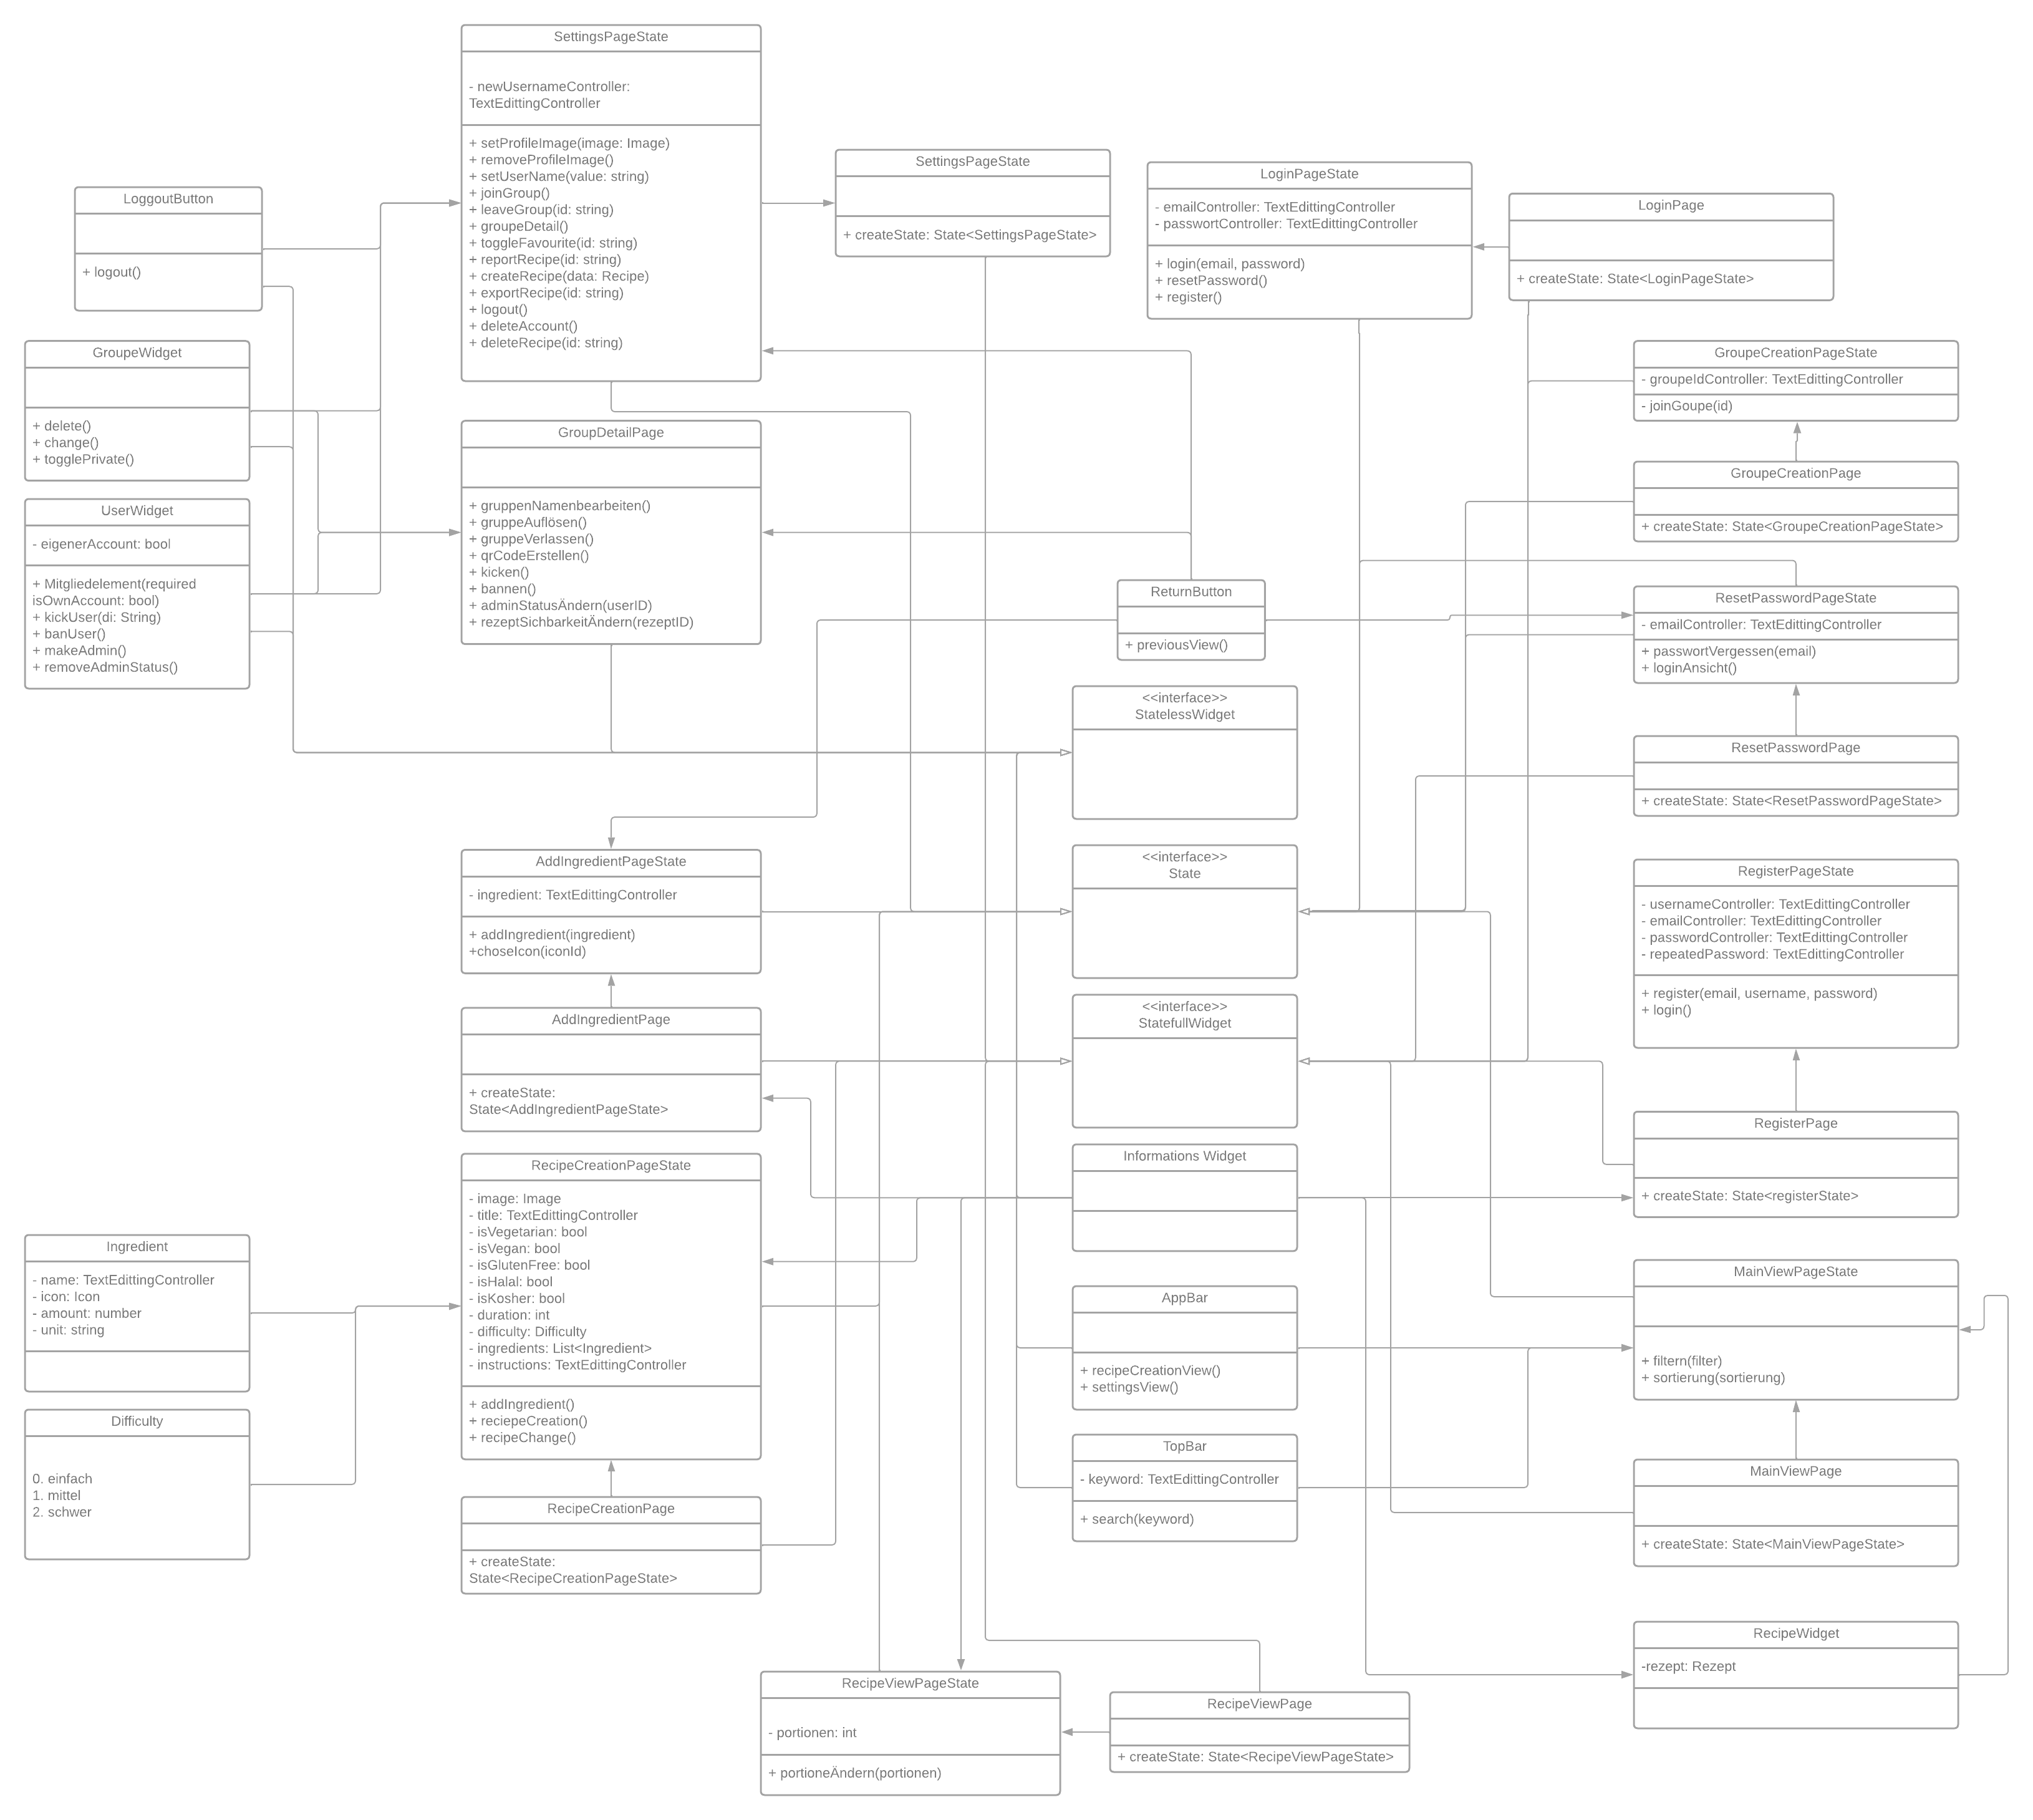
\includegraphics[width = \textwidth]{images/presentationLayer/presentationLayer.png}
    \caption{Klassendiagramm des Presentation Layer}
    \label{fig:presentation-layer}
\end{figure}

\newpage
\subsubsection{Recipe Creation Page}
Die Klassen beinhaltet alle nötigen Funktionen und Attribute um die Rezept-Erstell-Ansicht darzustellen.\newline


\paragraph{RecipeCreationPageState}
\textbf{Attributes}
\begin{itemize}
    \item image(blob): Hochgeladenes Bild welches den anderen Nutzern in der Rezeptansicht angezeigt werden soll.
    \item title(varchar(64) - not null): Die eingegebene Zeichenkette für den Titel des Rezepts. Die Zeichenkette kann maximal 64 Zeichen lang sein und muss ausgefüllt sein.
    \item is\_Vegetarian(bool): Der vom Nutzer angegebene Boolean ob das \gls{label} Vegetarisch dem Leser angezeigt werden soll. Ist standartmäßig auf false.
    \item is\_Vegan(bool): Der vom Nutzer angegebene Boolean ob das \gls{label} Vegan dem Leser angezeigt werden soll. Ist standartmäßig auf false.
    \item is\_GlutenFree(bool): Der vom Nutzer angegebene Boolean ob das \gls{label} Glutenfrei dem Leser angezeigt werden soll.  Ist standartmäßig auf false.
    \item is\_Halal(bool): Der vom Nutzer angegebene Boolean ob das \gls{label} Halal dem Leser angezeigt werden soll.  Ist standartmäßig auf false.
    \item is\_Kosher(bool): Der vom Nutzer angegebene Boolean ob das \gls{label} Koscher dem Leser angezeigt werden soll.  Ist standartmäßig auf false.
    \item duration(int - not null): Die vom Nutzer eingegebene Ganzzahl, welche die Zubereitunszeit in Minuten angibt. Muss angegeben werden.
    \item difficulty(Difficulty - not null: Die vom Nutzer ausgewählte \gls{schwierigkeit} des Rezepts. Muss angegeben werden.
    \item ingredients(Ingredients[]): Eine Liste an Ingerdients, welche in der AddIngredientPage erstellt wurde:
    \item instructions(text - not null: Die vom Nutzer angegeben Zeichenkette für die Beschreibung des Rezepts. Muss angegeben werden.
\end{itemize}

\textbf{Methods}
\begin{itemize}
    \item addIngredient(): Die Page AddIngredientPage wird aufgerufen.
    \item recipeSave(): Die Methode ruft, abhängig davon ob das Rezept neu erstellt wird oder nur verändert wurde, entweder recipeCreation() oder recipeChange() auf.
\end{itemize}

\begin{figure}[htp]
    \centering
    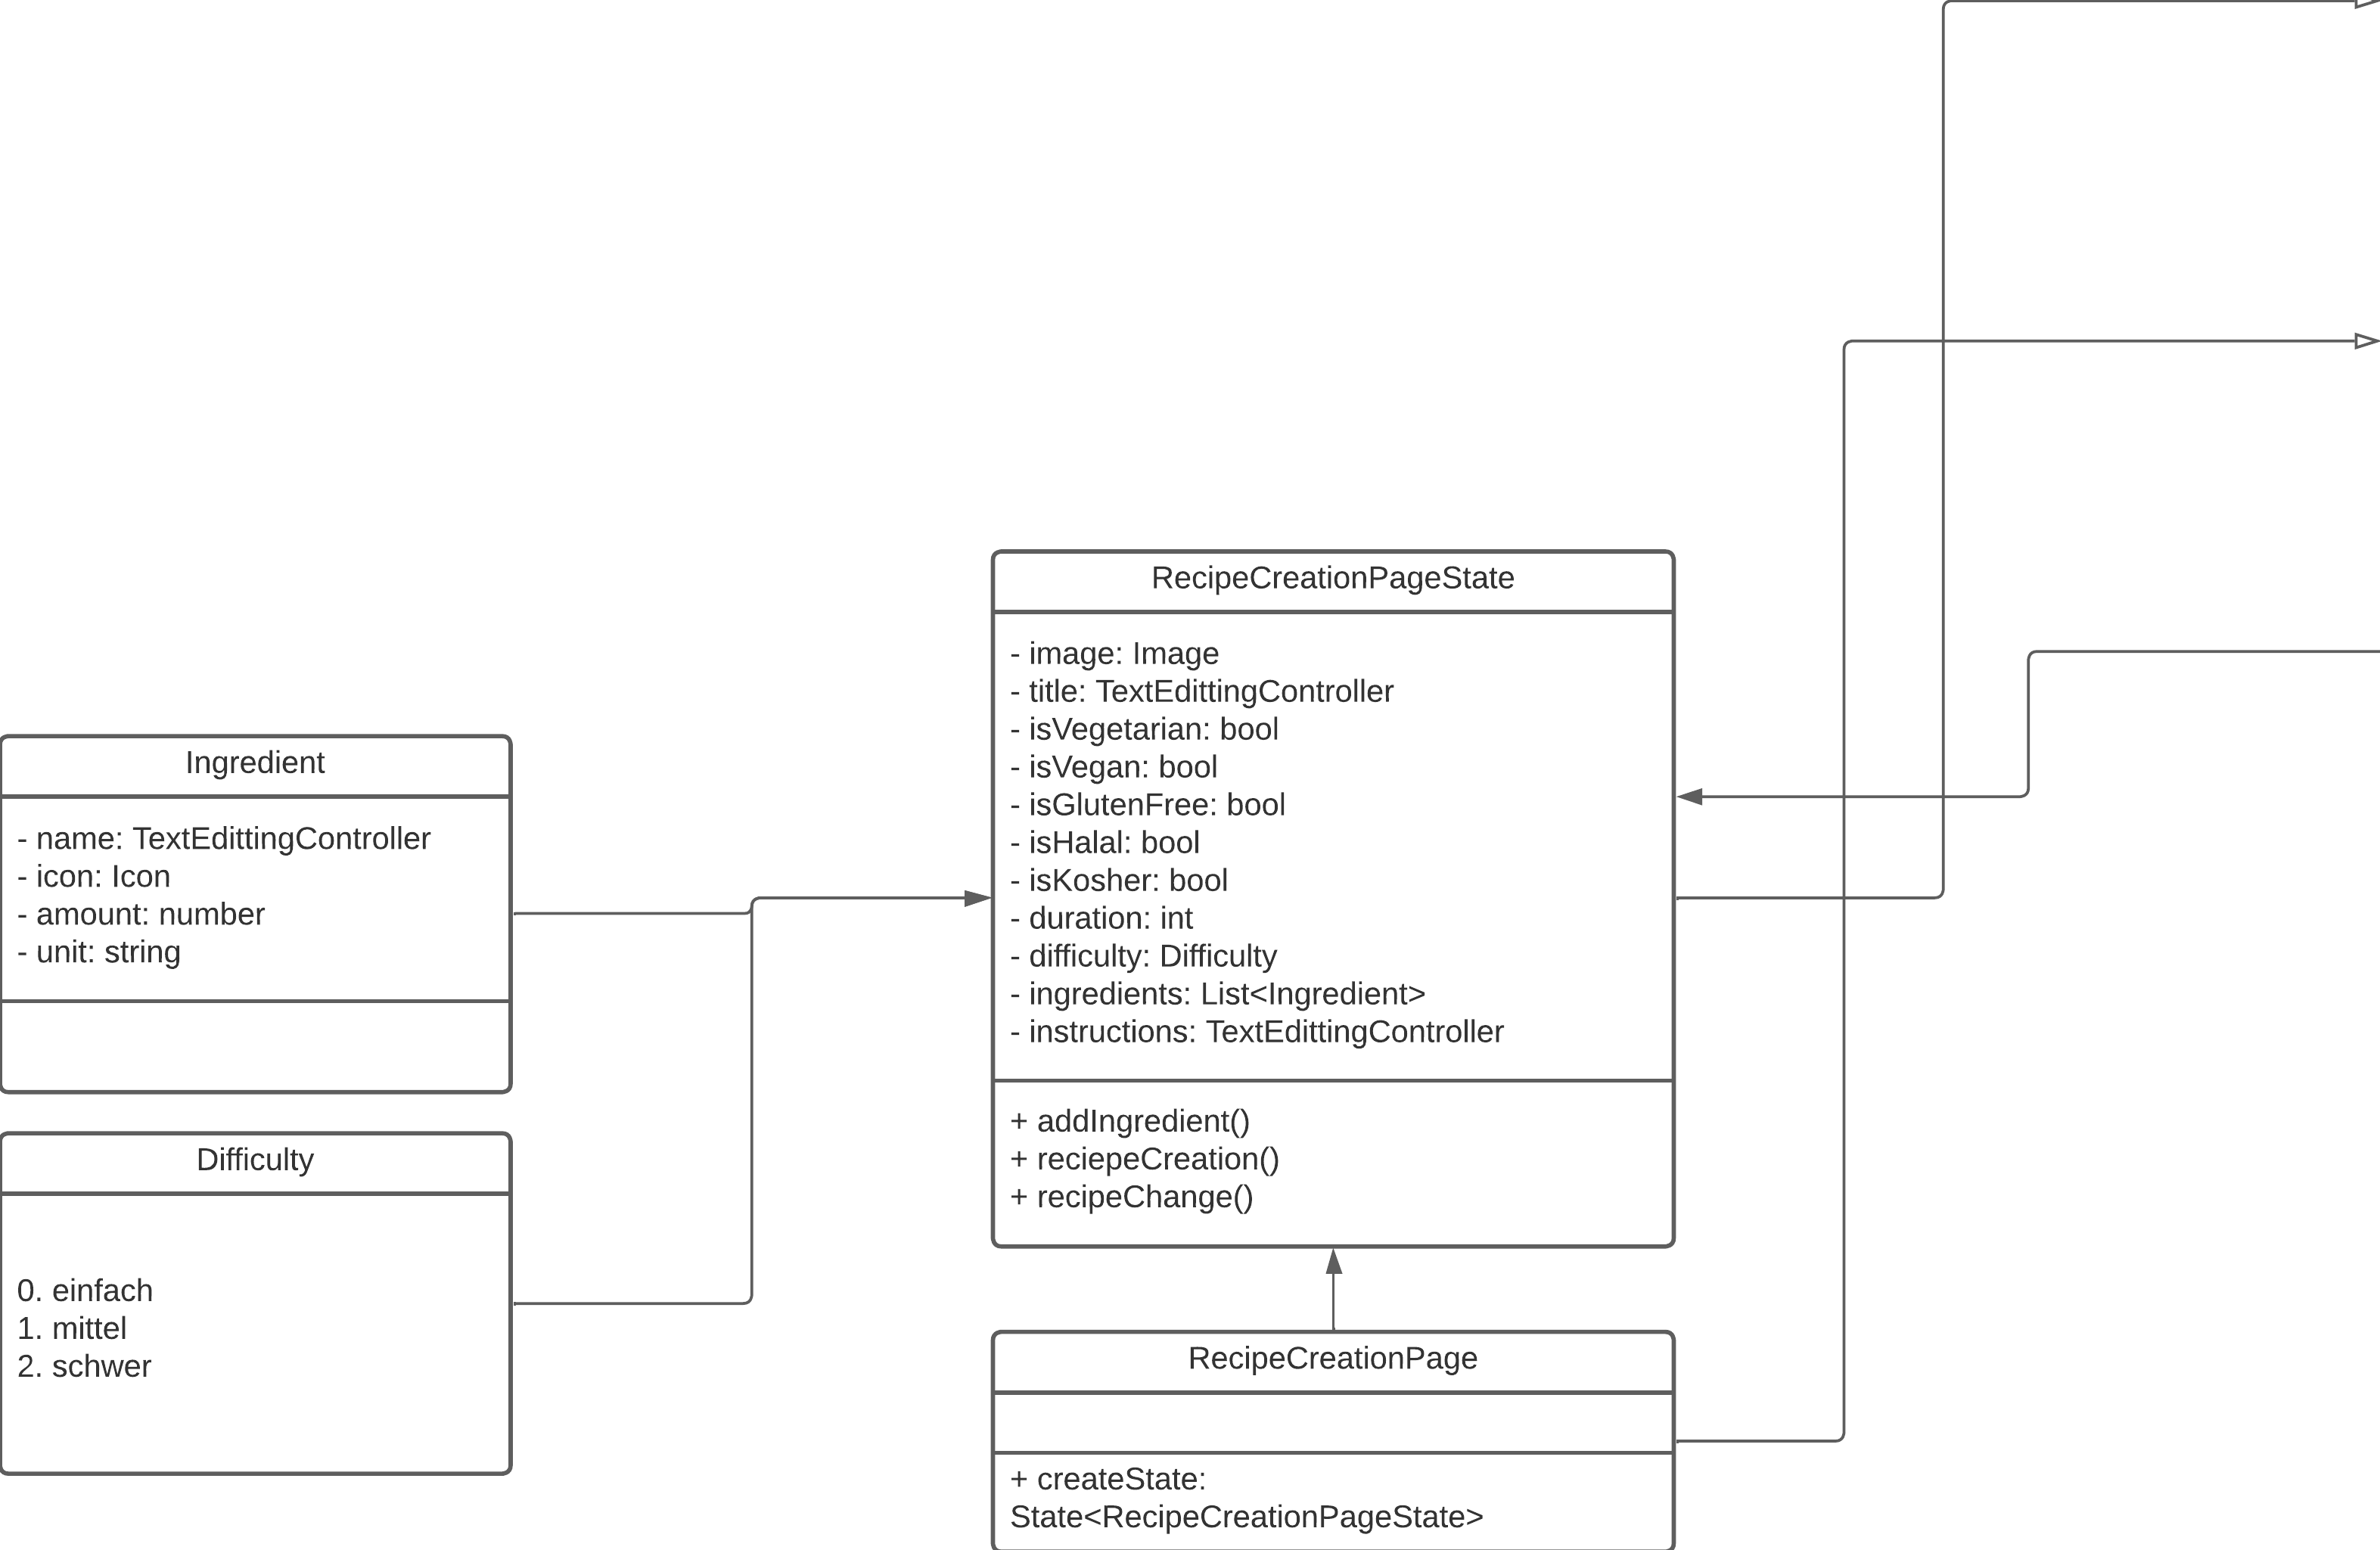
\includegraphics[height = 50mm]{images/presentationLayer/recipeCreationPage.png}
    \caption{RecipeCreationPage}
\end{figure}


\newpage

\subsubsection{Hauptansicht}
Die Klassen beinhaltet alle nötigen Funktionen und Attribute um die Hauptansicht darzustellen.\newline

\paragraph{MainViewPage}
\textbf{Methods}
\begin{itemize}
    \item createState: State<MainViewPageState> - Konstruktor für den MainViewPageState.
\end{itemize}

\paragraph{MainViewPageState}
\textbf{Methods}
\begin{itemize}
    \item filtering(filter: FilteringMethods) - Alle Rezepte werden dem Filterkriterium gefiltert.
    \item sorting(sort: SortingMethods) - Alle Rezepte werden nach dem Sortierkriterium sortiert.
\end{itemize}

\paragraph{TopBar}
\textbf{Attributes}
\begin{itemize}
    \item keyword: TextEdittingController - Eingegebene Zeichenkette durch den Nutzer für die Suche.
\end{itemize}
\textbf{Methodes}
\begin{itemize}
    \item search(keyword: TextEdittingController) - Durchsucht alle Rezepte um gibt jene aus, welche Rezepttitel zu dem Schlagwort passen.
\end{itemize}

\paragraph{AppBar}
\textbf{Methodes}
\begin{itemize}
    \item recipeCreationView() - Die Rezept-erstell-Ansicht wird aufgerufen.
    \item settingsView() - Die Einstellungsansicht wird aufgerufen.
\end{itemize}

\paragraph{RecipeWidget}
\textbf{Attributes}
\begin{itemize}
    \item recipe: Recipe - Das mit dem Widget dargestellte Rezept.
\end{itemize}
\textbf{Methodes}
\begin{itemize}
    \item RecipeWidget(recipe: Recipe - notNull) - Konstruktor für ein Recipe Widget. Ein Rezept muss angegeben werden.
\end{itemize}

\paragraph{InformationWidget}
\textbf{Attributes}
\begin{itemize}
    \item information: InformationKategories - Gibt an welche Information in dem Widget dargestellt werden soll.
    \item text: string - Der Text der in dem Widget angezeigt werden kann.
\end{itemize}

\textbf{Methodes}
\begin{itemize}
    \item InformationWidget(information: InformationKategories - notNull, text: string) - Konstruktor für ein Information Widget. Eine Information Kategorie muss angegeben werden.
\end{itemize}

\paragraph{SortingMethods}
Ein Enum der alle Sortierung Methoden beinhält.
\textbf{Content}
\begin{itemize}
    \item  alphabetical - Die Rezepte werden alphabetisch sortiert.
    \item  difficulty - Die Rezepte werden nach dem \gls{schwierigkeit}{Schwierigkeitsgrad} sortiert.
    \item  date - Die Rezepte werden nach dem Hinzufüge Datum sortiert.
\end{itemize}

\paragraph{FilteringMehods}
Ein Enum der alle Filter Methoden beinhält.
\textbf{Content}
\begin{itemize}
    \item favorits - Die Rezepte werden nach Favoriten gefiltert.
    \item difficultyEasy - Die Rezepte werden nach dem \glslink{schwierigkeit}{Schwierigkeitsgrad} einfach gefiltert.
    \item difficultyMedium - Die Rezepte werden nach dem \glslink{schwierigkeit}{Schwierigkeitsgrad} mittel gefiltert.
    \item difficultyHard - Die Rezepte werden nach dem \glslink{schwierigkeit}{Schwierigkeitsgrad} schwer gefiltert.
    \item labelVegetarian - Die Rezepte werden nach dem \gls{label} vegetarisch gefiltert.
    \item labelVegan - Die Rezepte werden nach dem \gls{label} vegan gefiltert.
    \item labelGlutenFree - Die Rezepte werden nach dem \gls{label} Gluten frei gefiltert.
    \item labelHalal - Die Rezepte werden nach dem \gls{label} halal gefiltert.
    \item labelKoscher - Die Rezepte werden nach dem \gls{label} koscher gefiltert.
\end{itemize}

\paragraph{InformationKategories}
Ein Enum der alle Information Kategorien beinhält.
\textbf{Content}
\begin{itemize}
    \item duration - Das Widget gibt an.
    \item difficultyEasy - Das Widget gibt den \glslink{schwierigkeit}{Schwierigkeitsgrad} einfach an.
    \item difficultyMedium - Das Widget gibt den \glslink{schwierigkeit}{Schwierigkeitsgrad} mittel an.
    \item difficultyHard - Das Widget gibt den \glslink{schwierigkeit}{Schwierigkeitsgrad} schwer an.
    \item labelVegetarian - Das Widget gibt das \gls{label} vegetarisch an.
    \item labelVegan - Das Widget gibt das \gls{label} vegan an.
    \item labelGlutenFree - Das Widget gibt das \gls{label} Gluten frei an.
    \item labelHalal - Das Widget gibt das \gls{label} halal an.
    \item labelKoscher - Das Widget gibt das \gls{label} koscher an.
\end{itemize}

\begin{figure}[htp]
    \begin{minipage}
        [t]{0.49\textwidth}
        \centering
        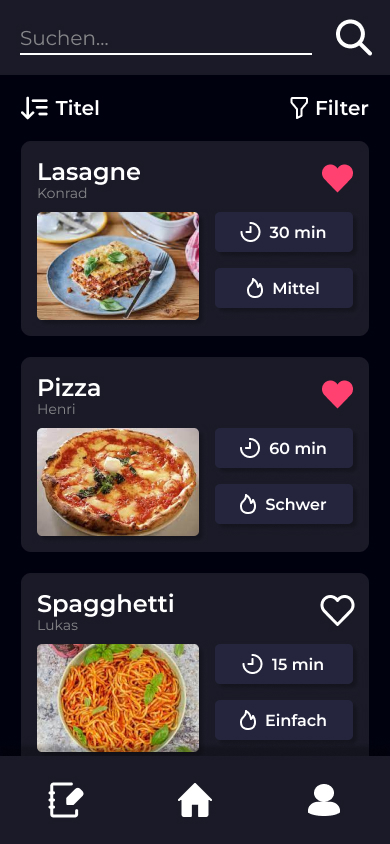
\includegraphics[height=80mm]{images/Presentation-layer/MainView.jpg}
        \caption{Hauptansicht}
    \end{minipage}
    \begin{minipage}
        [t]{0.49\textwidth}
        \centering
        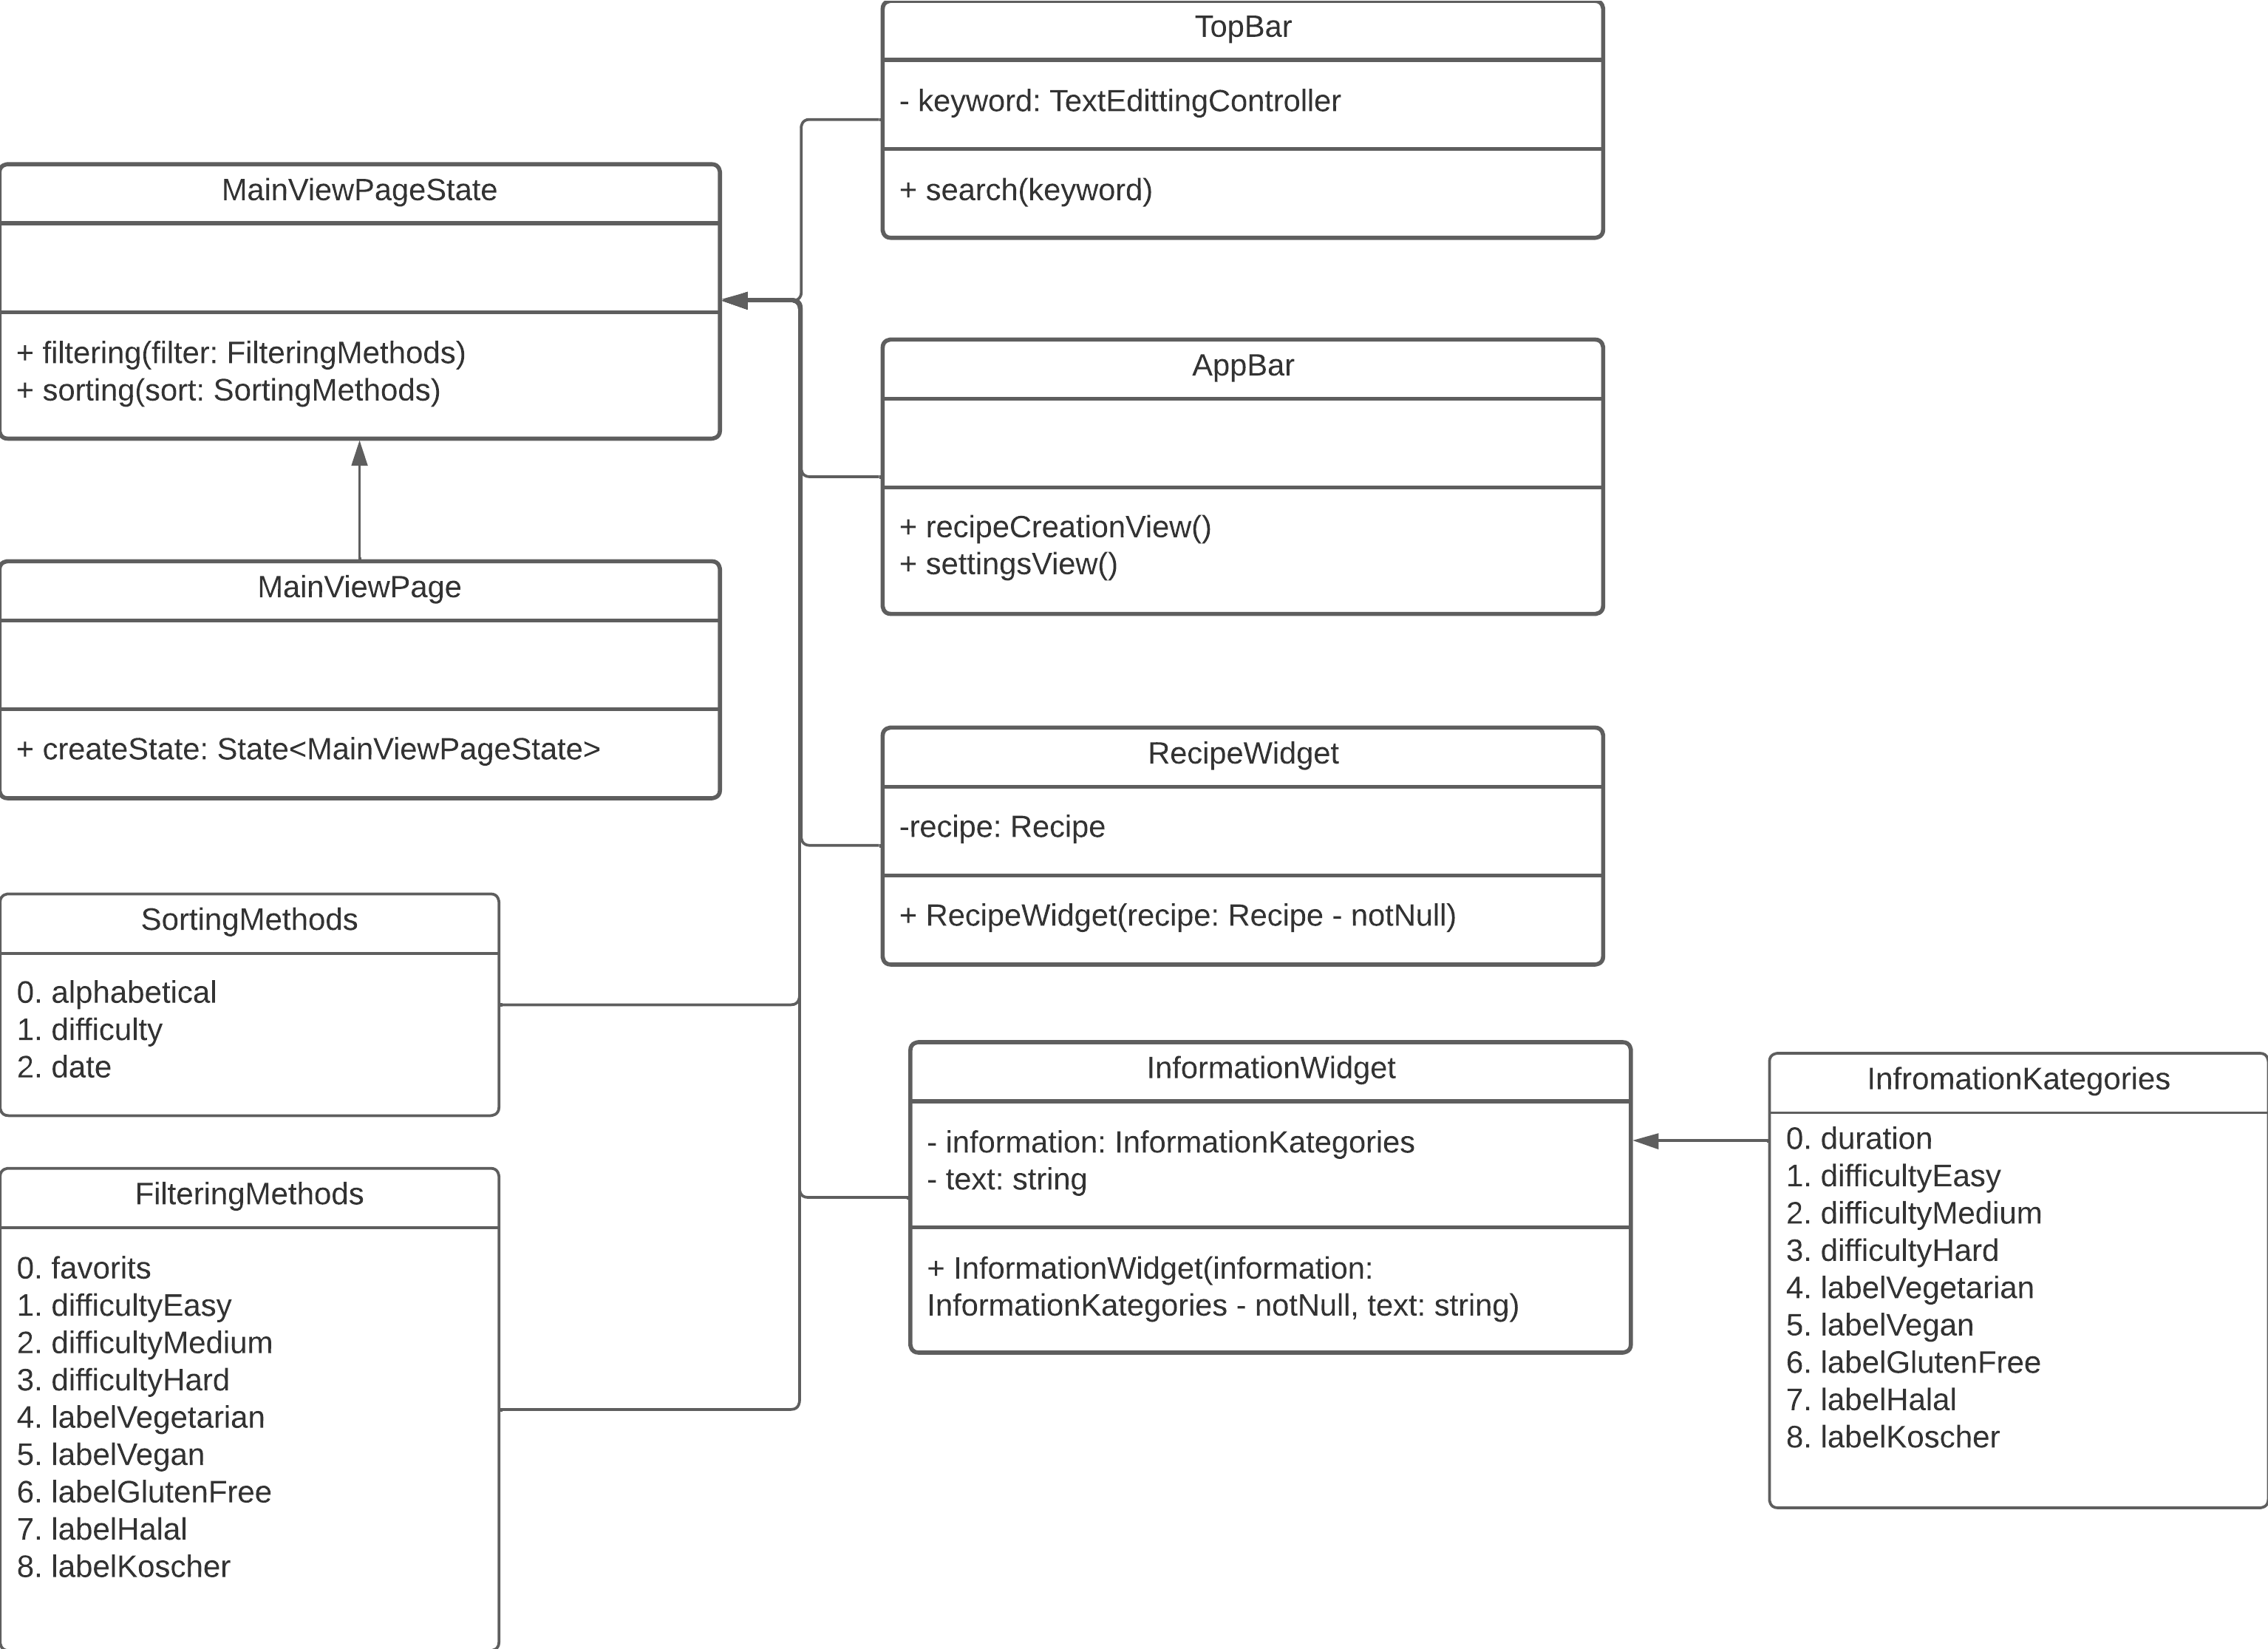
\includegraphics[width=0.95\textwidth]{images/Presentation-layer/MainViewClass.png}
        \caption{Klassen für Hauptansicht}
    \end{minipage}
\end{figure}

\newpage

\section{REST-Webservice}

\subsection{Server}
\subsection*{Attribute}
\paragraph{port: number} Durch das Attribut port lässt sich einstellen auf welchen Port Anfragen an den Server zulässig sind.
Port ist vom Type number.
\paragraph{firebaseCredentials: any}
\paragraph{express: express.Application}
\paragraph{app: App}
\paragraph{}

\subsection*{Methode}
\paragraph{public <<create>> constructor(): void}
\paragraph{public start(): void}
\paragraph{private connectToDatabase(): void}
\paragraph{private connectToFirebase(): void}
\paragraph{private createServer(): void}


\subsection{App}
\subsubsection*{Attribute}
\paragraph{app: express.Application}
\paragraph{authentificationRoutes: AuthentificationRouter}
\paragraph{recipeRoutes: RecipeRouter}
\paragraph{groupRoutes: GroupRouter}
\paragraph{userRoutes: UserRouter}
\paragraph{IngredientRouter}

\subsubsection*{Methode}
\paragraph{public <<create> constructor(express.Application): void}
\paragraph{private initializeMiddleware(): void}
\paragraph{private initializeRoutes(): void}
\paragraph{privtate initializeErrorHandlers(): void}

\subsection{Router}
\subsubsection{AbstractRouter}
\subsubsection*{Attribute}
\paragraph{protected router: express.Router}
\paragraph{protected controller: AbstractController}
\paragraph{protected checkAuthorization: CheckAuthorization}
\paragraph{protected checkAuth: any}

\subsubsection*{Methode}
\paragraph{public <<create>> constructor(): void}
\paragraph{protected abstract setupRoutes(): void}
\paragraph{public getRouter(): express.Router}

\subsubsection{AuthentificationRouter}
\subsubsection*{Methode}
\paragraph{public <<create>> constructor(): void}
\paragraph{protected setupRoutes(): void}

\subsubsection{RecipeRouter}
\subsubsection*{Methode}
\paragraph{public <<create>> constructor(): void}
\paragraph{protected setupRoutes(): void}

\subsubsection{GroupRouter}
\subsubsection*{Methode}
\paragraph{public <<create>> constructor(): void}
\paragraph{protected setupRoutes(): void}

\subsubsection{UserRouter}
\subsubsection*{Methode}
\paragraph{public <<create>> constructor(): void}
\paragraph{protected setupRoutes(): void}

\subsubsection{IngredientRouter}
\subsubsection*{Methode}
\paragraph{public <<create>> constructor(): void}
\paragraph{protected setupRoutes(): void}

\subsection{Middleware}
\subsubsection{CheckAuthorization}
\subsubsection*{Methode}
\paragraph{authChecker(req: any, res, any, next: any): void}

\subsection{Controller}
\subsubsection{AbstractController}
\subsubsection*{Methode}


\subsubsection{AuthentificationController}
\subsubsection*{Methode}
\paragraph{public userRegister(req: any, res: any, next: any): void}
\paragraph{public userLogin(req: any, res: any, next: any): void}
\paragraph{userResetPassword(req: any, res: any, next: any): void}
\paragraph{}

\subsubsection{RecipeController}
\subsubsection*{Methode}
\paragraph{public recipePost(req: any, res: any, next: any): void}
\paragraph{public recipeDelete(req: any, res: any, next: any): void}
\paragraph{public recipePatch(req: any, res: any, next: any): void}
\paragraph{public recipeGet(req: any, res: any, next: any): void}
\paragraph{public recipeGetAll(req: any, res: any, next: any): void}
\paragraph{public recipeSetFavorite(req: any, res: any, next: any): void}
\paragraph{public recipeGetByGroup(req: any, res: any, next: any): void}

\subsubsection{GroupController}
\subsubsection*{Methode}
\paragraph{public groupPost(req: any, res: any, next: any): void}
\paragraph{public groupDelete(req: any, res: any, next: any): void}
\paragraph{public groupGetById(req: any, res: any, next: any): void}
\paragraph{public groupPatch(req: any, res: any, next: any): void}
\paragraph{public groupJoin(req: any, res: any, next: any): void}
\paragraph{public groupLeave(req: any, res: any, next: any): void}

\subsubsection{UserController}
\subsubsection*{Methode}
\paragraph{public userDelete(req: any, res: any, next: any): void}
\paragraph{public userPatch(req: any, res: any, next: any): void}

\subsubsection{IngredientController}
\subsubsection*{Methode}
\paragraph{ingredientGetAll(req: any, res: any, next: any): void}

\newpage

\section{Datenbank}
Die zugrundeliegende Datenbank soll möglichst nah an unseren Entitäten orientiert sein, um inkonsistente Daten zu vermeiden. Daher wird für das Projekt die Datenbank "PostgreSQL" verwendet. Sie unterstützt relationale Datenformate und ist daher optimal für unsere Anforderungen geeignet. Zudem ist sie Open-Source und kostenlos und erfreut sich seit 35 Jahren großer Beliebtheit.
\subsection{Datenbankschema}
\begin{figure}[htp]
    \centering
    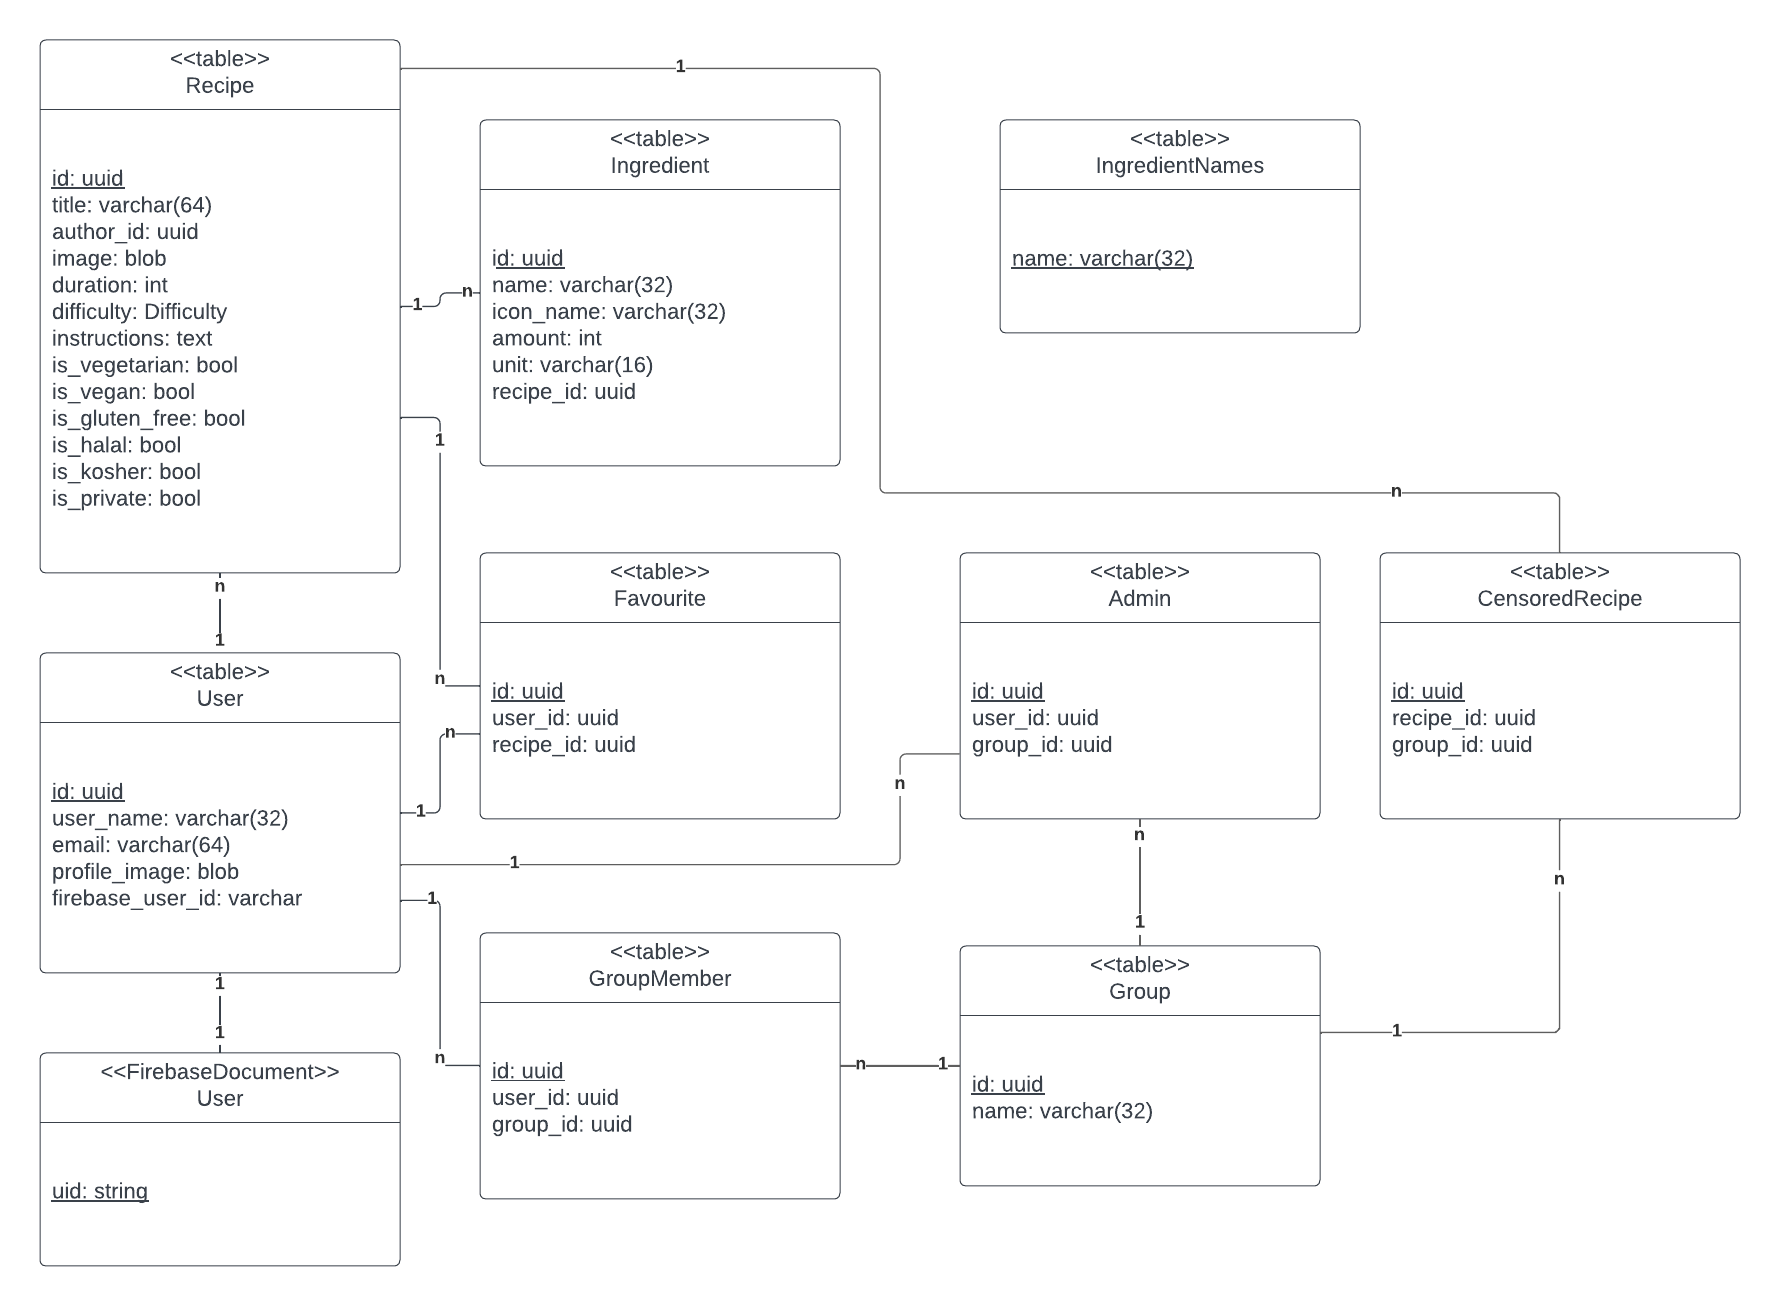
\includegraphics[width = \linewidth]{images/Database/schema.png}
    \caption{Datenbankschema}
\end{figure}
Im Datenbankschema werden die einzelnen Entitäten der App abgebildet. Die einzelnen Tabellen werden nun genauer erläutert.
\newpage
\subsubsection{Recipe}
Die Tabelle "Recipe" enthält die Rezepte und besitzt die folgenden Attribute:
\paragraph{id (uuid - primary key):} Die Id stellt den Primärschlüssel des Rezepts dar und muss daher eindeutig und nicht leer sein. Der Datentyp ist \Gls{uuid}. Sie wird automatisch generiert.
\paragraph{title (varchar(64) - not null):} Der Titel des Rezepts. Der Datentyp ist \Gls{varchar}. Er darf nicht leer und maximal 64 Zeichen lang sein.
\paragraph{author\_id (uuid - not null, foreign key):} Hierbei handelt es sich um die Id des Autors des Rezepts als Fremdschlüssel. Sie darf nicht leer sein und der Datentyp ist \Gls{uuid}, da es sich um eine Id handelt.
\paragraph{image (blob):} Das Bild des Rezepts in binär Code. Der Datentyp ist \Gls{blob}.
\paragraph{duration (int - not null):} Die Zubereitungszeit des Rezepts in Minuten. Der Datentyp ist Integer. Sie darf nicht leer sein.
\paragraph{difficulty (Difficulty - not null):} Die Schwierigkeit des Rezepts, die nicht leer sein darf. Der Datentyp "Difficulty" ist ein Enum, mit den Werten "easy", "medium" und "hard".
\paragraph{instructions (text - not null):} Die Zubereitungsanleitung des Rezepts, die nicht leer sein darf. Der Datentyp ist Text, was einer unbegrenzten Zeichenkette entspricht.
\paragraph{is\_vegetarian (bool - not null):} Gibt an, ob das \Gls{label} "Vegetarisch" aktiviert ist. Der Datentyp ist Boolean und darf nicht leer sein.
\paragraph{is\_vegan (bool - not null):} Gibt an, ob das \Gls{label} "Vegan" aktiviert ist. Der Datentyp ist Boolean und darf nicht leer sein.
\paragraph{is\_gluten\_free (bool - not null):} Gibt an, ob das \Gls{label} "Glutenfrei" aktiviert ist. Der Datentyp ist Boolean und darf nicht leer sein.
\paragraph{is\_halal (bool - not null):} Gibt an, ob das \Gls{label} "Halal" aktiviert ist. Der Datentyp ist Boolean und darf nicht leer sein.
\paragraph{is\_kosher (bool - not null):} Gibt an, ob das \Gls{label} "Koscher" aktiviert ist. Der Datentyp ist Boolean und darf nicht leer sein.
\newpage
\subsubsection{Ingredient}
Die Tabelle "Ingredient" enthält die Zutaten, die den eizelnen Rezepten zugeordnet sind und besitzt die folgenden Attribute:
\paragraph{id (uuid - primary key):} Die Id stellt den Primärschlüssel der Zutat dar und muss daher nicht leer und eindeutig sein. Der Datentyp ist \Gls{uuid}. Sie wird automatisch generiert.
\paragraph{name (varchar(32) - not null):} Der Name der Zutat. Der Datentyp ist \Gls{varchar}. Er darf nicht leer und maximal 32 Zeichen lang sein.
\paragraph{icon\_name (varchar(32))} Der Name des Icons, das die Zutat repräsentiert. Der Datentyp ist \Gls{varchar}. Er ist maximal 32 Zeichen lang.
\paragraph{amount (int - not null):} Die Menge der Zutat in der jeweiligen Einheit. Sie darf nicht leer sein und der Datentyp ist Integer.
\paragraph{unit (varchar(16)):} Die Einheit der Zutat. Der Datentyp ist \Gls{varchar}. Sie ist maximal 16 Zeichen lang und optional.
\paragraph{recipe\_id (uuid - not null, foreign key):} Hierbei handelt es sich um die Id des Rezepts, zu dem die Zutat gehört, als Fremdschlüssel. Sie darf nicht leer sein und der Datentyp ist \Gls{uuid}, da es sich um eine Id handelt.
\newpage
\subsubsection{IngredientNames}
Die Tabelle "IngredientNames" enthält lediglich die Namen der Zutaten, die in der Vorschlagsliste beim Zutaten erstellen angezeigt werden. Sie besitzt die folgenden Attribute:
\paragraph{name (varchar(32) - primary key):} Der Name der Zutat. Der Datentyp ist \Gls{varchar}. Es handelt sich um den Primärschlüssel und der Name muss daher eindeutig und nicht leer sein.
\newpage
\subsubsection{User}
Die Tabelle "User" enthält die Benutzer der App und besitzt die folgenden Attribute:
\paragraph{id (uuid - primary key):} Die Id stellt den Primärschlüssel des Benutzers dar und muss daher eindeutig und nicht leer sein. Der Datentyp ist \Gls{uuid}. Sie wird automatisch generiert.
\paragraph{user\_name (varchar(32) - not null):} Der Benutzername des Benutzers. Der Datentyp ist \Gls{varchar}. Er darf nicht leer und maximal 32 Zeichen lang sein.
\paragraph{email (varchar(64) - not null):} Die E-Mail-Adresse des Benutzers. Der Datentyp ist \Gls{varchar}. Sie darf nicht leer und maximal 64 Zeichen lang sein.
\paragraph{profile\_image (blob):} Das Profilbild des Benutzers in binär Code. Der Datentyp ist \Gls{blob}.
\paragraph{firebase\_user\_id (varchar - not null, unique)} Die Id des Benutzers, die in der Firebase Datenbank hinterlegt ist. Der Datentyp ist \Gls{varchar}. Sie muss eindeutig und nicht leer sein. Sie dient als Fremdschlüssel über die Datenbank hinweg zu Firebase.
\newpage
\subsubsection{Favourite}
Die Tabelle "Favourite" repräsentiert die Many-To-Many-Beziehung zwischen den Benutzern und den Rezepten, die sie favorisiert haben. Sie besitzt die folgenden Attribute:
\paragraph{id (uuid - primary key):} Die Id stellt den Primärschlüssel der Beziehung dar und muss daher eindeutig und nicht leer sein. Der Datentyp ist \Gls{uuid}. Sie wird automatisch generiert.
\paragraph{user\_id (uuid - not null, foreign key):} Hierbei handelt es sich um die Id des Benutzers, der das Rezept favorisiert hat, als Fremdschlüssel. Sie darf nicht leer sein und der Datentyp ist \Gls{uuid}, da es sich um eine Id handelt.
\paragraph{recipe\_id (uuid - not null, foreign key):} Hierbei handelt es sich um die Id des Rezepts, das favorisiert wurde, als Fremdschlüssel. Sie darf nicht leer sein und der Datentyp ist \Gls{uuid}, da es sich um eine Id handelt.
\newpage
\subsubsection{Group}
Die Tabelle "Group" enthält die Gruppen bzw. Squads und besitzt die folgenden Attribute:
\paragraph{id (uuid - primary key):} Die Id stellt den Primärschlüssel der Gruppe dar und muss daher eindeutig und nicht leer sein. Der Datentyp ist \Gls{uuid}. Sie wird automatisch generiert.
\paragraph{name (varchar(32) - not null):} Der Name der Gruppe. Der Datentyp ist \Gls{varchar}. Er darf nicht leer und maximal 32 Zeichen lang sein.
\newpage
\subsubsection{GroupMember}
Die Tabelle "GroupMember" repräsentiert die Many-To-Many-Beziehung zwischen den Gruppen und den Benutzern, die Mitglied der Gruppe sind. Sie besitzt die folgenden Attribute:
\paragraph{id (uuid - primary key):} Die Id stellt den Primärschlüssel der Beziehung dar und muss daher eindeutig und nicht leer sein. Der Datentyp ist \Gls{uuid}. Sie wird automatisch generiert.
\paragraph{user\_id (uuid - not null, foreign key):} Hierbei handelt es sich um die Id des Benutzers, der Mitglied der Gruppe ist, als Fremdschlüssel. Sie darf nicht leer sein und der Datentyp ist \Gls{uuid}, da es sich um eine Id handelt.
\paragraph{group\_id (uuid - not null, foreign key):} Hierbei handelt es sich um die Id der Gruppe, zu der der Benutzer gehört, als Fremdschlüssel. Sie darf nicht leer sein und der Datentyp ist \Gls{uuid}, da es sich um eine Id handelt.
\newpage
\subsubsection{Admin}
Die Tabelle "Admin" repräsentiert die Many-To-Many-Beziehung zwischen den Gruppen und den Benutzern, die Administratoren der Gruppe sind. Sie besitzt die folgenden Attribute:
\paragraph{id (uuid - primary key):} Die Id stellt den Primärschlüssel der Beziehung dar und muss daher eindeutig und nicht leer sein. Der Datentyp ist \Gls{uuid}. Sie wird automatisch generiert.
\paragraph{user\_id (uuid - not null, foreign key):} Hierbei handelt es sich um die Id des Benutzers, der Administrator der Gruppe ist, als Fremdschlüssel. Sie darf nicht leer sein und der Datentyp ist \Gls{uuid}, da es sich um eine Id handelt.
\paragraph{group\_id (uuid - not null, foreign key):} Hierbei handelt es sich um die Id der Gruppe, zu der der Benutzer gehört, als Fremdschlüssel. Sie darf nicht leer sein und der Datentyp ist \Gls{uuid}, da es sich um eine Id handelt.
\newpage
\subsubsection{CensoredRecipe}
Die Tabelle "CensoredRecipe" repräsentiert die Many-To-Many-Beziehung zwischen den Gruppen und den Rezepten, die die jeweiligen Administratoren zensiert haben. Sie besitzt die folgenden Attribute:
\paragraph{id (uuid - primary key):} Die Id stellt den Primärschlüssel der Beziehung dar und muss daher eindeutig und nicht leer sein. Der Datentyp ist \Gls{uuid}. Sie wird automatisch generiert.
\paragraph{recipe\_id (uuid - not null, foreign key):} Hierbei handelt es sich um die Id des Rezepts, das zensiert wurde, als Fremdschlüssel. Sie darf nicht leer sein und der Datentyp ist \Gls{uuid}, da es sich um eine Id handelt.
\paragraph{group\_id (uuid - not null, foreign key):} Hierbei handelt es sich um die Id der Gruppe, zu der der Administrator gehört, als Fremdschlüssel. Sie darf nicht leer sein und der Datentyp ist \Gls{uuid}, da es sich um eine Id handelt.
\newpage

\section{Ablaufbeschreibung}

\section{Klassenindex}
\subsection{Client-Klassen}
\subsection{Server-Klassen}

\section{Glossar}
\printglossary[style=altlist]
\end{document}